\documentclass[8pt]{beamer}
\mode<presentation>
{
  \setbeamercovered{transparent}
  \setbeamertemplate{navigation symbols}{} % no navigation bar
}
\usepackage[T1]{fontenc}
\usepackage[utf8]{inputenc}
\usepackage{lmodern}
\usepackage{listings}
\usepackage{color}

\definecolor{grey}{rgb}{0.8, 0.8, 0.8}
\definecolor{darkblue}{rgb}{0.0, 0.18, 0.39}
\setbeamercolor{frametitle}{fg=darkblue}

\lstset{frame=tb,
  aboveskip=1mm,
  belowskip=1mm,
  showstringspaces=false,
  columns=flexible,
  basicstyle={\tiny\ttfamily\color{darkblue}},
  breaklines=true,
  breakatwhitespace=true,
  rulecolor=\color{grey}
}
\begin{document}

\begin{frame}
\frametitle{PicDat -- Instruction}
\begin{figure}
	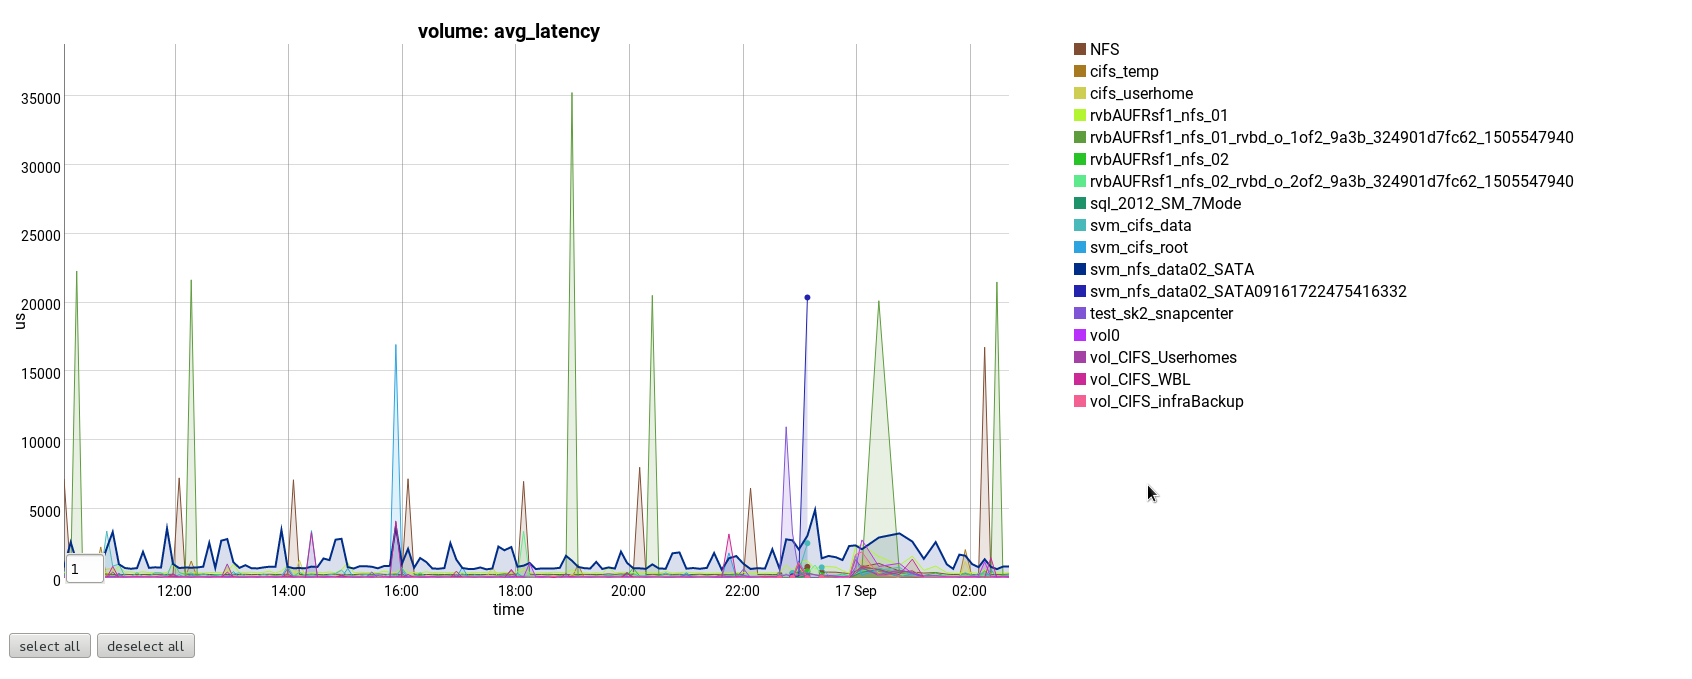
\includegraphics[width=\textwidth]{../images/PicDat_normal.png}
\end{figure}
The aim of PicDat is to provide better insight to performance data from NetApp controllers. The command line tool is able to visualize data from both PerfStat output and ASUP files.

PicDat selects some counters of such files which are typically sufficient for the analysis and writes them to several csv tables. Then it generates a HTML file using a JavaScript library called dygraphs to visualize those tables. Open the HTML in a browser to get your performance charts.
\end{frame}

\begin{frame}
\frametitle{Running PicDat}
You can run PicDat without any parameters. After you startet it, it'll ask you for some performance input. Additionally, PicDat will ask you to enter a directory for its results. Be aware, that content might become overwritten if this directory is not empty. After this, PicDat will start working. 
\bigskip

Alternatively, you can pass input and output specifications as command line parameters. Therefore, use the options \textcolor{darkblue}{\texttt{-\,-inputfile}} and \textcolor{darkblue}{\texttt{-\,-outputdir}} or \textcolor{darkblue}{\texttt{-i}} and \textcolor{darkblue}{\texttt{-o}} respectively.
\smallskip

Another available command line option is the \textcolor{darkblue}{\texttt{-\,-debug}} or \textcolor{darkblue}{\texttt{-d flag}}. It specifies the filtering level for command line output. Pass it together with a string out of those: \texttt{debug, info, warning, error, critical}
Default is \texttt{info}.
\smallskip

If you wand to redirect the command line output into a log file for further analysis, use the flag \textcolor{darkblue}{\texttt{-\,-logfile}} or \textcolor{darkblue}{\texttt{-l}}. This will create a picdat.log file inside your output directory.
\smallskip

By default, PicDat sorts the most data series by relevance. This means, the graph with the highest sum of values will be displayed at the top of a chart's legend. If you rather wants them to be sorted alphanumeric, use the flag \textcolor{darkblue}{\texttt{-\,-sortbyname}} or \textcolor{darkblue}{\texttt{-s}}.
\bigskip

To get an overview about all command line option, try option \textcolor{darkblue}{\texttt{-\,-help}} or  \textcolor{darkblue}{\texttt{-h}}.
\end{frame}

\begin{frame}
\frametitle{Input format}
As mentioned, PicDat can handle two different types of performance data.
\bigskip

If you want to visualize \textcolor{darkblue}{\textbf{PerfStat data}}, you have following options: Either you can pass single PerfStat data files (they have to end with \textbf{.data} or \textbf{.out}) or you can pass a \textbf{directory}, containing such files. Furthermore, you can pass a \textbf{.zip} file containing PerfStat output. If you transmit a single file, be aware, that some meta data which are usually packed together with PerfStats, will not be readable. If you transmit several PerfStats (within a directory or zip), PicDat will generate \textbf{one HTML} with charts \textbf{for each PerfStat}. 
\bigskip

\textcolor{darkblue}{\textbf{ASUP}} data are usually packed in tar files with file extension \textbf{.tgz}. You can pass them as input in a whole. It is also possible to transmit the unpacked tars, i.e. a \textbf{directory}. There is nothing as a single file transmission available, because PicDat needs at least two files, a CM-STATS-HOURLY-INFO.XML and a CM-STATS-HOURLY-DATA.XML file for its analysis. 

Working with ASUPs, it might be useful to visualize data for several consecutive ASUP files together. To do so, just pack \textbf{several ASUP .tgz archives into one directory} and pass the directory to PicDat. PicDat will stick the results for the different data files together. This means, different from visualizing PerfStats, only \textbf{one HTML for all data} will be generated. So don't mess around and pack ASUP files into one folder, which don't belong together! Don't mix nodes.
\end{frame}

\begin{frame}[fragile]
\frametitle{Run example}
This is how a run could look like on your command line:
\smallskip

\begin{lstlisting}
python picdat.py -i"</path/to/input>" -o"</path/to/output>" 
2018-03-09 12:00:35,195 INFO: inputfile: </path/to/input>, outputdir: </path/to/output>
2018-03-09 12:00:35,196 INFO: Prepare directory...
2018-03-09 12:00:35,202 INFO: Running PicDat in PerfStat mode
2018-03-09 12:00:35,202 INFO: Did not find a console.log file to extract perfstat's cluster and node name.
2018-03-09 12:00:35,202 INFO: Read data...
2018-03-09 12:00:37,796 INFO: Planned number of iterations was executed correctly.
2018-03-09 12:00:37,798 INFO: Create csv tables...
2018-03-09 12:00:37,799 INFO: Wrote chart values into /path/to/output/tables/aggregate_total_transfers_chart_values.csv
2018-03-09 12:00:37,799 INFO: Wrote chart values into /path/to/output/tables/processor_processor_busy_chart_values.csv
2018-03-09 12:00:37,799 INFO: Wrote chart values into /path/to/output/tables/volume_read_ops_chart_values.csv
2018-03-09 12:00:37,801 INFO: Wrote chart values into /path/to/output/tables/volume_write_ops_chart_values.csv
2018-03-09 12:00:37,801 INFO: Wrote chart values into /path/to/output/tables/volume_other_ops_chart_values.csv
2018-03-09 12:00:37,801 INFO: Wrote chart values into /path/to/output/tables/volume_total_ops_chart_values.csv
2018-03-09 12:00:37,802 INFO: Wrote chart values into /path/to/output/tables/volume_avg_latency_chart_values.csv
2018-03-09 12:00:37,802 INFO: Wrote chart values into /path/to/output/tables/volume_read_data_chart_values.csv
2018-03-09 12:00:37,802 INFO: Wrote chart values into /path/to/output/tables/volume_write_data_chart_values.csv
2018-03-09 12:00:37,807 INFO: Wrote chart values into /path/to/output/tables/sysstat_1sec_percent_chart_values.csv
2018-03-09 12:00:37,819 INFO: Wrote chart values into /path/to/output/tables/sysstat_1sec_MBs_chart_values.csv
2018-03-09 12:00:37,828 INFO: Wrote chart values into /path/to/output/tables/sysstat_1sec_IOPS_chart_values.csv
2018-03-09 12:00:37,830 INFO: Wrote chart values into /path/to/output/tables/statit_disk_statistics_chart_values.csv
2018-03-09 12:00:37,831 INFO: Create html file...
2018-03-09 12:00:37,833 INFO: Generated html file at /path/to/output/charts.html
2018-03-09 12:00:37,843 INFO: Done. You will find charts under: </path/to/output>
\end{lstlisting}
\smallskip

General usage: 
\smallskip
\begin{lstlisting}
picdat [--help] [--sortbyname] [--inputfile "input"] [--outputdir "output"] [--debug "level"] [--logfile]
\end{lstlisting}
\end{frame}

\begin{frame}
\frametitle{Interactive charts -- legend}
The Job of PicDat is to pick and visualize some of the various information given with the input. The charts.html files contains several labeled charts offering some interaction. 

\begin{figure}
	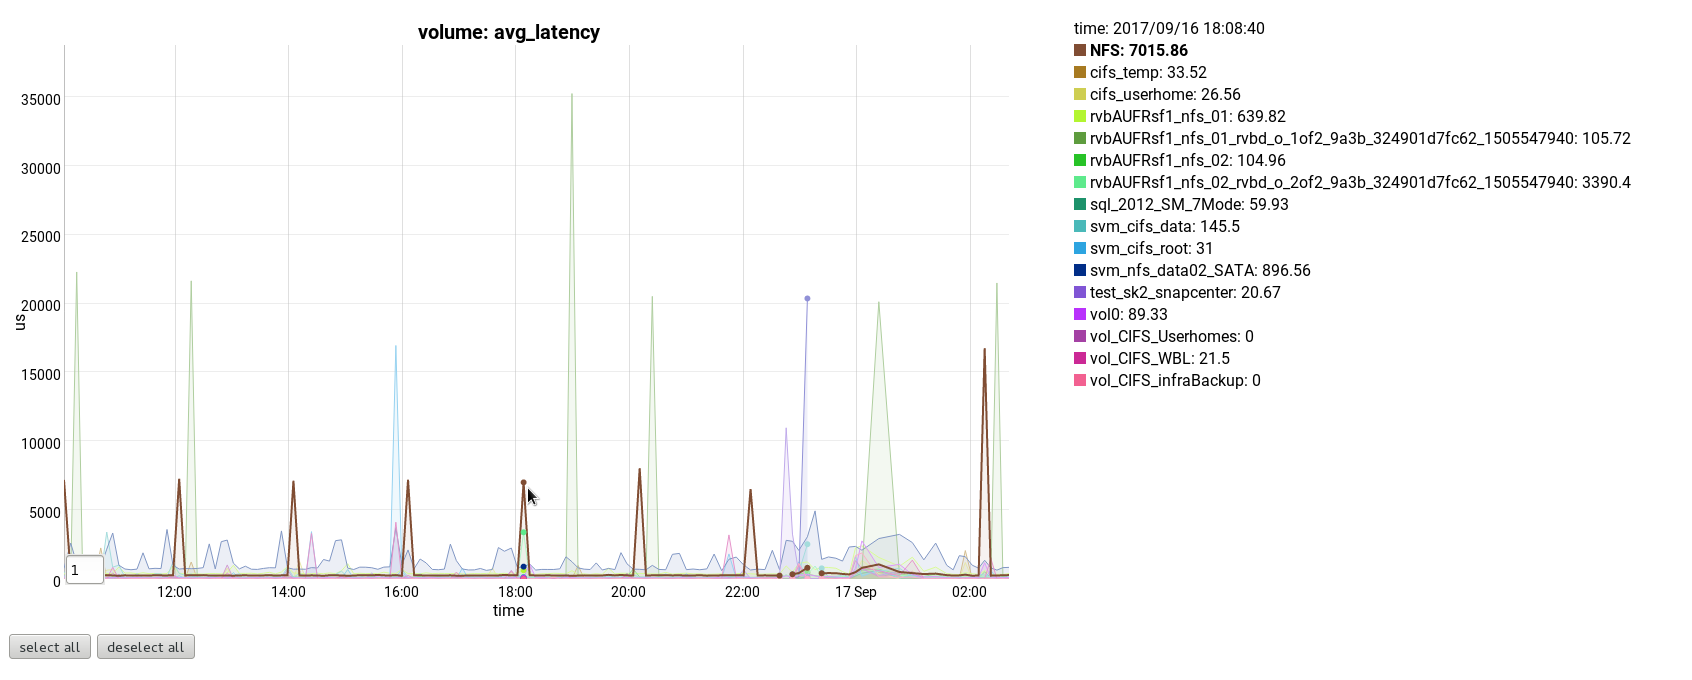
\includegraphics[width=\textwidth]{../images/PicDat_highlight2.png}
\end{figure}

Mouse-over them to display the values in the legend. You'll notice as well, that the graph, your cursor is next, will be highlighted. The corresponding entry in the legend will be highlighted similtaneously.
\end{frame}

\begin{frame}
\frametitle{Interactive charts -- legend} 
\begin{figure}
	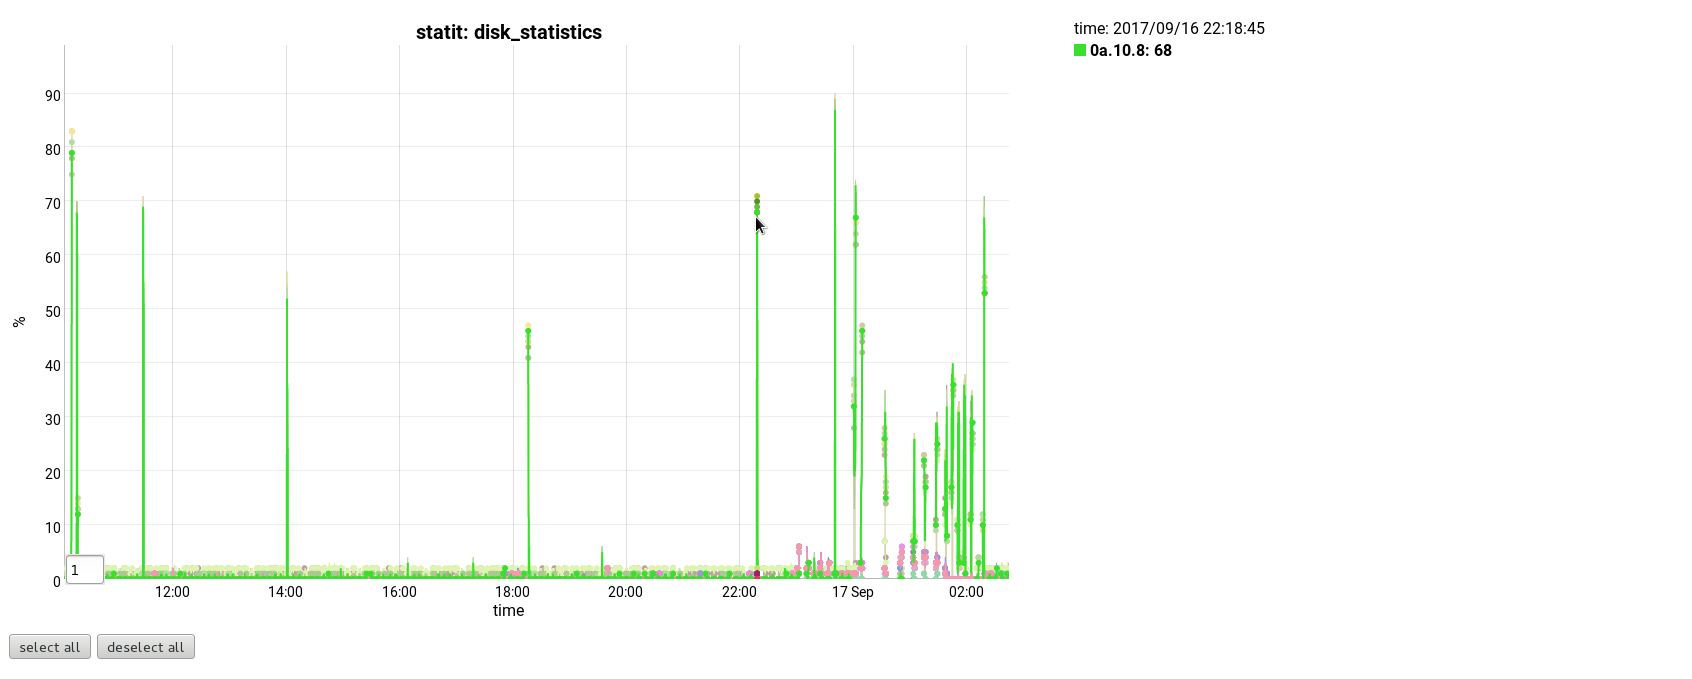
\includegraphics[width=\textwidth]{../images/PicDat_singleValue.png}
\end{figure}

If there are so many graphs in one chart that the legend can't display them all without a scroll bar, the legend will change to display only one value at once as soon as your mouse enters the chart.
\end{frame}

\begin{frame}
\frametitle{Interactive charts -- zoom} 
\begin{figure}
	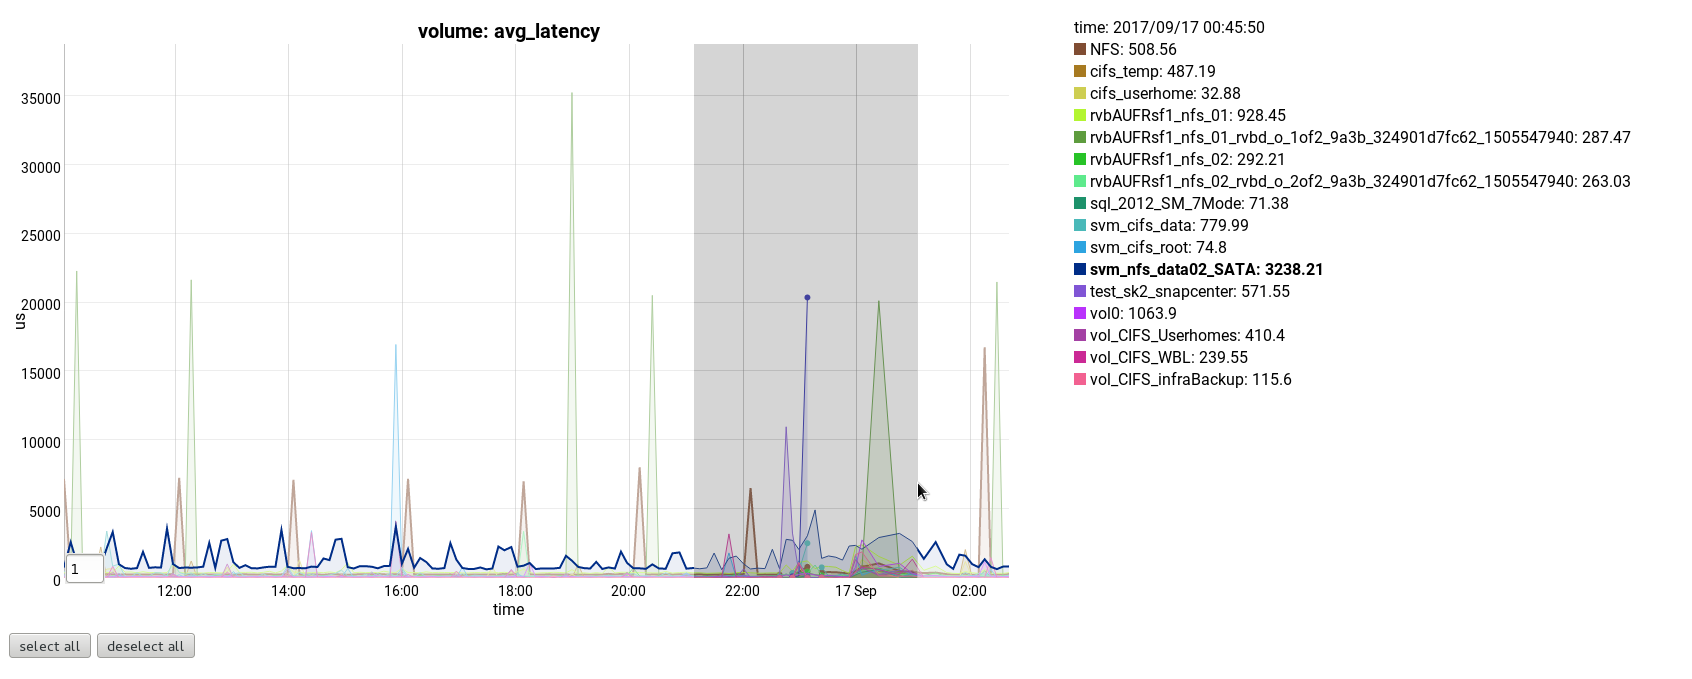
\includegraphics[width=\textwidth]{../images/PicDat_zoomVertical.png}
\end{figure}

To zoom inside the charts, just click and drag them in x or y direction. Once zoomed in, you can also change the displayed range by holding shift an click and drag again. To go back into original view, just double-click the chart.
\end{frame}

\begin{frame}
\frametitle{Interactive charts -- select and deselect} 
\begin{figure}
	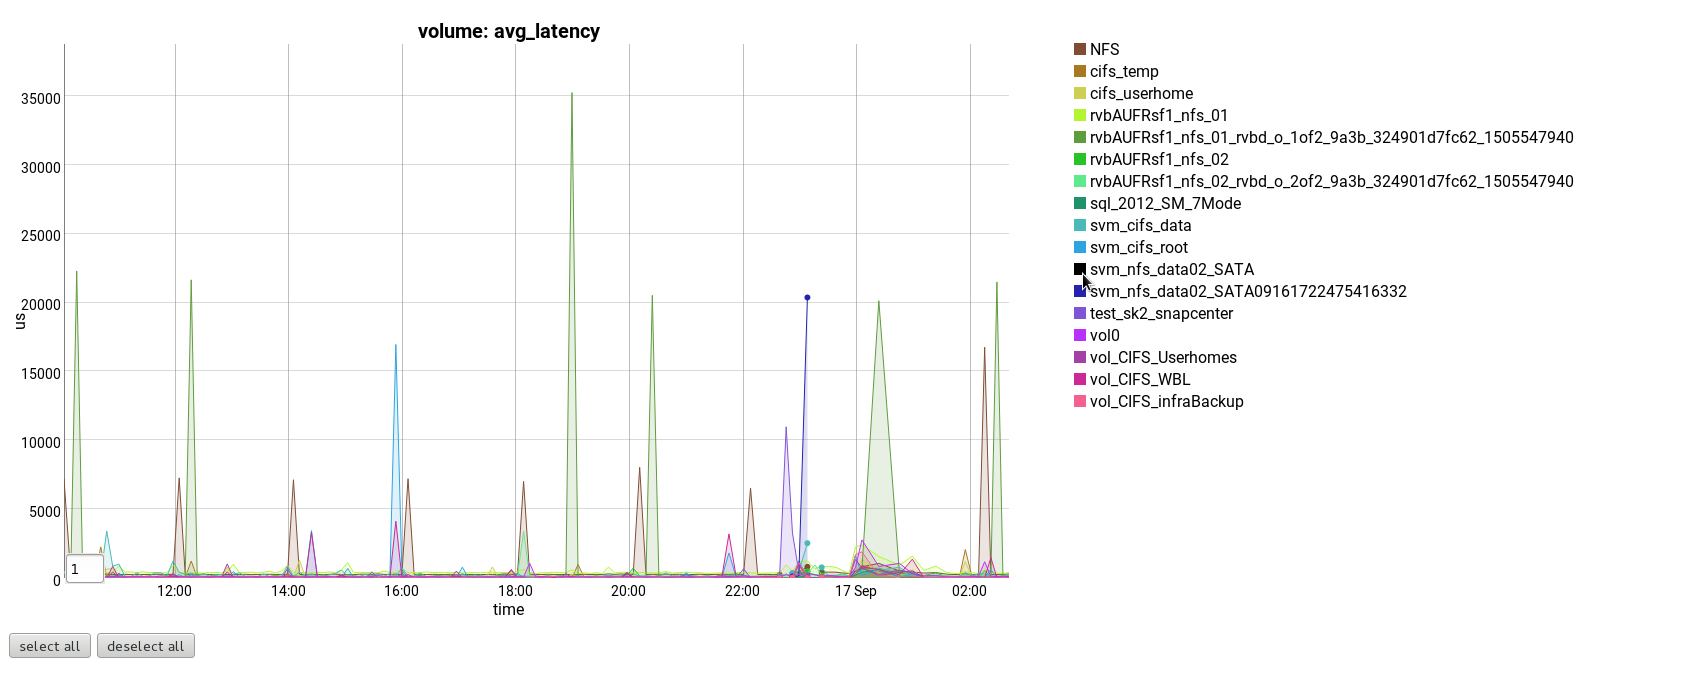
\includegraphics[width=\textwidth]{../images/PicDat_deselect.png}
\end{figure}

You might wish to take some graph lines out of view. Therefore, click one of the colored boxes inside the legend. It'll turn to black and the corresponding graph will disappear from sight. Click it again and the graph will come back. To select or deselect all lines at once, use the buttons beneath the chart.
Note, that disabled graphs disappear from the legend whereas your cursor is on the chart. Entries, belonging to graphs with a gap at the place your cursor recently is, will disappear as well. So don't be confused if the legend will bounce a bit as you move your mouse.
\end{frame}

\begin{frame}
\frametitle{Interactive charts -- rolling average} 
\begin{figure}
	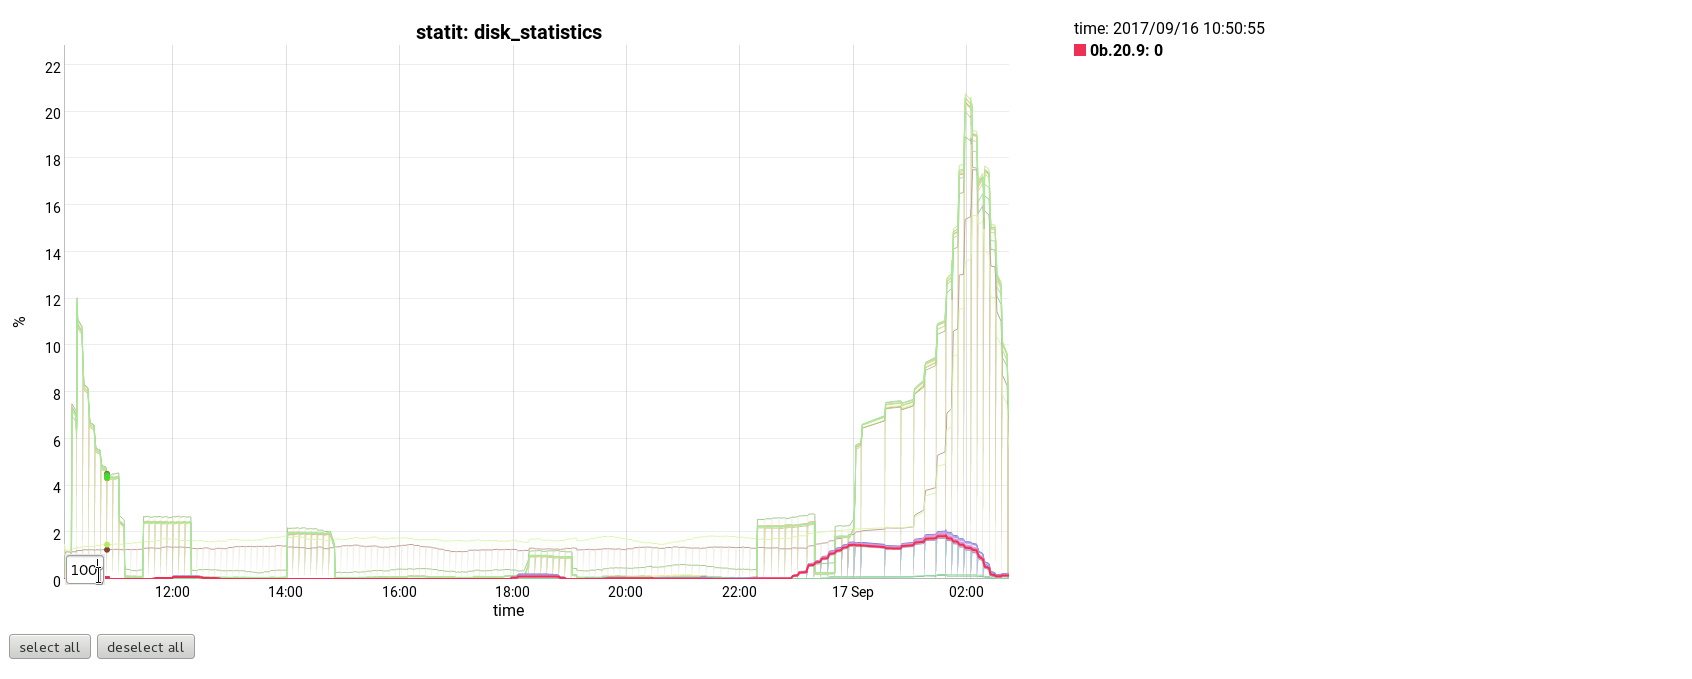
\includegraphics[width=\textwidth]{../images/PicDat_roller.png}
\end{figure}

If your values are very close and unsteady, you might get a better overview using a rolling average. Therefore, type a natural number into the small textfield appearing at the lower left corner of most charts. After hitting 'enter', the data will get averaged over this number of measuring points.
\end{frame}

\begin{frame}
\frametitle{Can't see any graphs?}
If you are running the charts.html from your file system, the Browsers Chrome and Internet Explorer/Edge are blocking external files for security reasons. So, the dygraph.js can't be loaded. To avoid this, use Firefox instead, use a local web server or try to change security settings.
If this is not the problem, make sure that dygraphs is available at all. A folder called 'dygraphs', containing the dygraph.js and dygraph.css, must be in the same location as your charts.html file.
\end{frame}

\end{document}
